%%
%% This is file `minimalexample',
%% generated with the docstrip utility.
%%
%% The original source files were:
%%
%% CASUS.dtx  (with options: `minimalexample')
%% ----------------:| --------------------------------------------------------
%% CASUS:           | Corporate Design for the CASUS project
%% Author:          | Tobias Schlemmer
%% E-mail:          | Tobias.Schlemmer@web.de
%% License:         | LaTeX files are released under the LaTeX Project Public License v1.3c or later
%%                  | Needed graphics files are not covered by this license.
%% See:             | http://www.latex-project.org/lppl.txt
%% 
\documentclass[english,aspectratio=169]{beamer}
\usepackage[utf8]{inputenc}
\usepackage[TS1,T1]{fontenc}
\usepackage{babel}
\usepackage{lmodern}
\usepackage{bm}
\usepackage{bbm}
\usepackage[framemethod=TikZ]{mdframed}

\usepackage[labelformat=empty,font=tiny,singlelinecheck=false]{caption}

\usepackage{mathtools}
\usepackage{multirow}
% Math notations are written in serif
\usefonttheme[onlymath]{serif}

\setbeamertemplate{navigation symbols}{}%remove navigation symbols

\usepackage{ragged2e}


\usepackage{pgfplots}

\pgfplotsset{compat=newest}
\usetikzlibrary{patterns}
\usepgfplotslibrary{fillbetween}

\let\tempone\itemize
\let\temptwo\enditemize
\renewenvironment{itemize}{\tempone\addtolength{\itemsep}{0.35\baselineskip}}{\temptwo}

\usepackage{xcolor}

% Bib
\usepackage[style=apa,backend=biber]{biblatex}
\addbibresource{bibliography.bib}
\renewcommand*{\bibfont}{\scriptsize}
\setbeamertemplate{bibliography item}{} % Remove icon from the list of references

% Argmin and argmax
\usepackage{amsmath}
\DeclareMathOperator*{\argmin}{arg\,min}
\DeclareMathOperator*{\argmax}{arg\,max}

% Left/right align figure
\usepackage[export]{adjustbox}

\usetheme{CASUS}
\title[\texttt{minterpy} docs]{%
  Introduction to \texttt{minterpy} docs}
\subtitle{\texttt{minterpy} dev. camp}
\author{Damar Wicaksono}

\def\blfootnote{\xdef\@thefnmark{}\@footnotetext}


%%%%%%%%%%%%%%%%%%%%%%%%%%%%%%%%%%%%%%%%%%%%%%%%%%%%%%%%%%%%%%%%%%%%%%%%%%%%%%
\begin{document}

\titleframe
\contentsframe

\section{Docs structure and organization}

%==============================================================================
\begin{frame}{}
\vfill
\centering

\begin{alertblock}{Disclaimer}
\centering
The docs is still work in-progress
\end{alertblock}

\vfill

\end{frame}


%==============================================================================
\begin{frame}{Thinking about the docs}
\footnotesize

\begin{columns}[onlytextwidth]

\begin{column}{0.5\textwidth}

Users and developers read the docs.

\vspace{0.5em}

If you think about \emph{when} the docs is read:
\begin{itemize}
    \item when you \emph{learn} about the code (for the first time or otherwise)
    \item when you are \emph{working} with it (advanced tasks, making contributions)
\end{itemize}

\vspace{0.5em}

If you think about the \emph{form of content}:
\begin{itemize}
    \item \emph{Practical steps}, with (runable) code examples
    \item \emph{Exposition}, with detailed description or explanation
\end{itemize}

\begin{exampleblock}<2>{}
    \centering
    There isn't \emph{one} docs, but \emph{four}
\end{exampleblock}

\end{column}

\begin{column}{0.5\textwidth}
    \begin{center}
    \includegraphics<2>[width=0.9\textwidth]{./figures/documentation-system-blank}
    \end{center}
\end{column}

\end{columns}
    
\end{frame}


%==============================================================================
\begin{frame}{Four categories of docs}
\footnotesize

\begin{columns}[onlytextwidth]

\begin{column}{0.5\textwidth}

the \texttt{minterpy} docs has four distinct categories:

\vspace{0.5em}

\begin{enumerate}
    \item Tutorials (getting started guides)
    \item How-to guides (for users and for contributors)
    \item Explanations/Fundamentals (explanation on mathematical background)
    \item (API) Reference
\end{enumerate}

\vspace{0.5em}

each with different purposes.

\end{column}

\begin{column}{0.5\textwidth}
    \begin{center}
    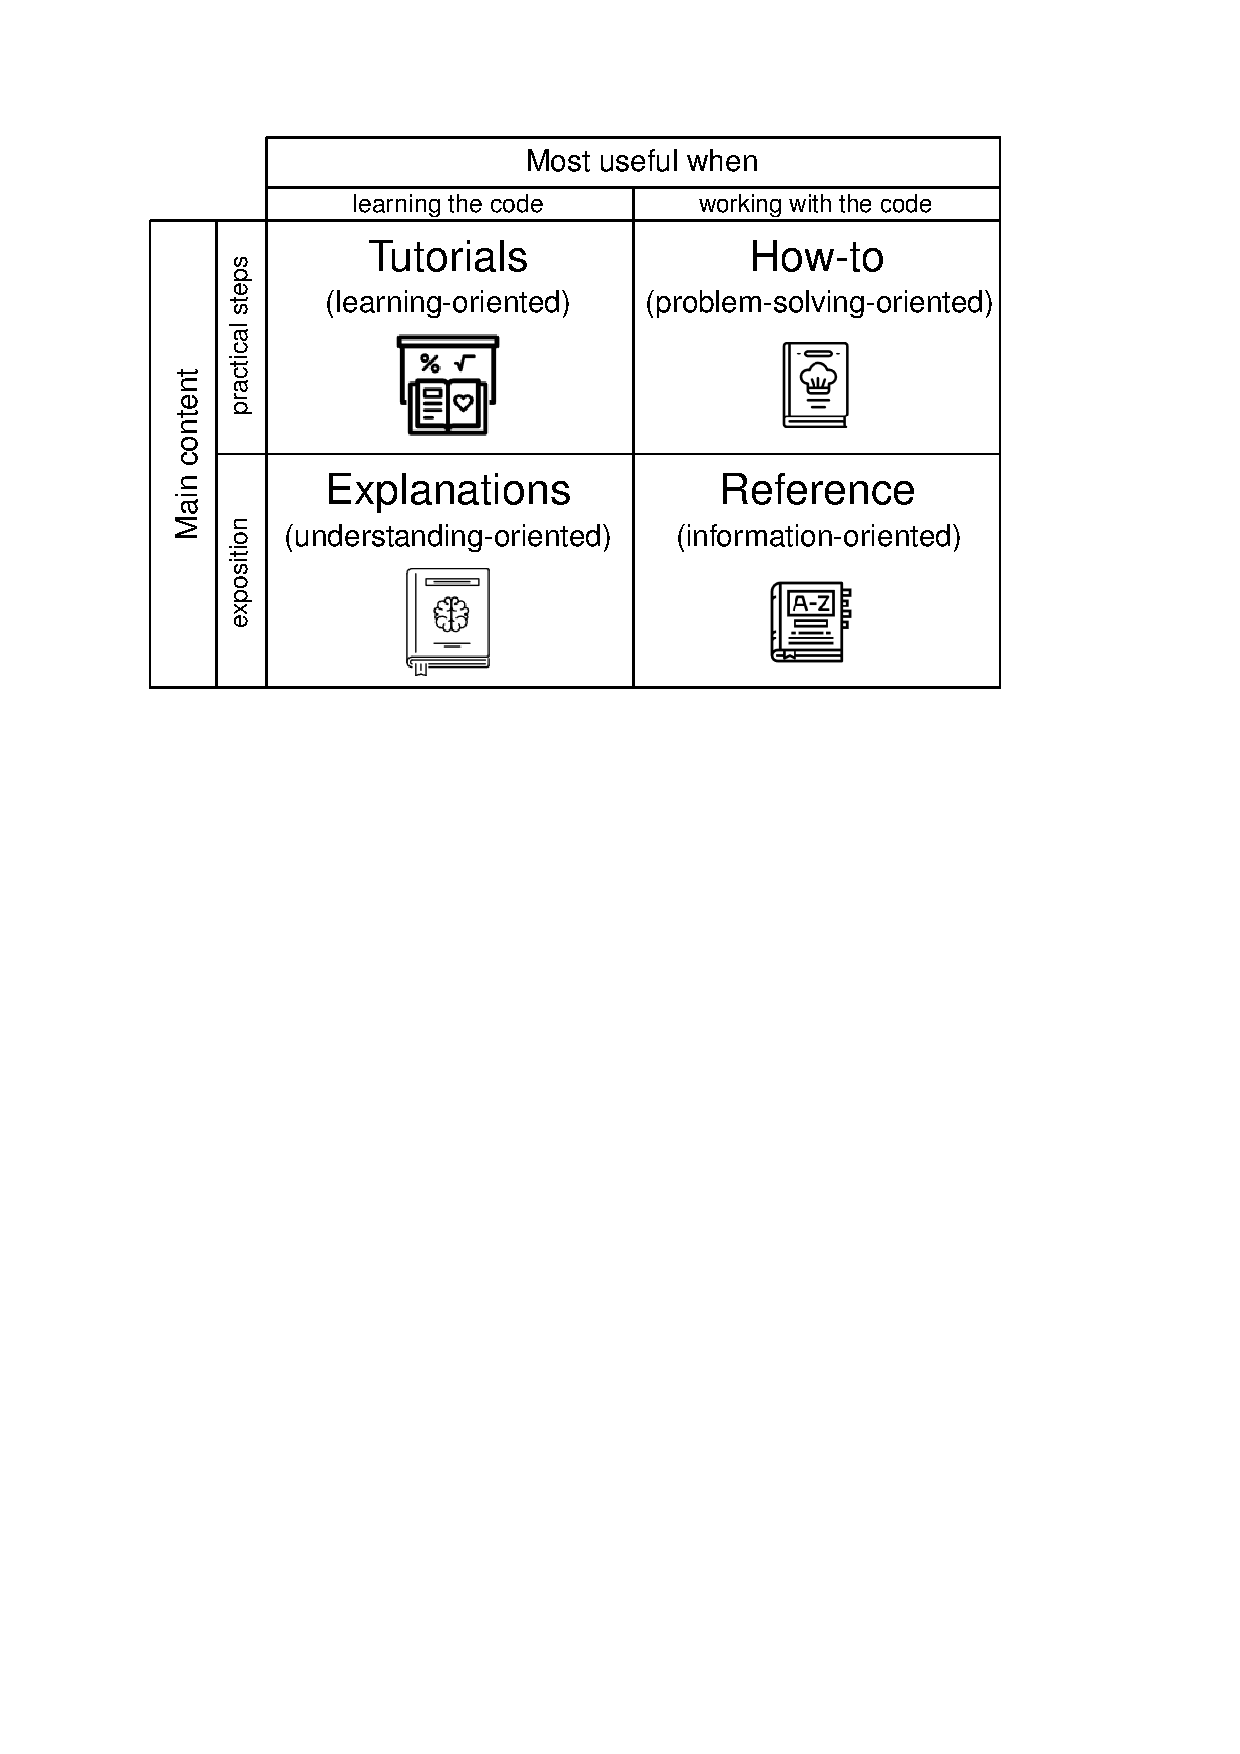
\includegraphics[width=0.9\textwidth]{./figures/documentation-system}
    \end{center}
    \vspace{-0.5em}
    \begin{exampleblock}{}
        \centering
        This documentation design principle is based on the Documentation System by Divio
        (\url{documentation.divio.com})
    \end{exampleblock}
\end{column}

\end{columns}

\end{frame}


%==============================================================================
\begin{frame}{Tutorials: learning-oriented docs}
\footnotesize
    
\begin{columns}[onlytextwidth]
    
\begin{column}{0.5\textwidth}

\begin{itemize}
    \item Think of tutorials as \emph{lessons} (in a self-study setting)
    \item Each should have a minimal (perhaps hypothetical) but non-trivial context\\
          and a quick outcome
    \item Important for onboarding users and developers;
          provide a first glimpse on \texttt{minterpy} functionalities and usage
    \item Tricky to write: must provide the \emph{why},
          write with progressive disclosure,
          think well about the curation 
\end{itemize}

\end{column}

\begin{column}{0.5\textwidth}
    \begin{center}
    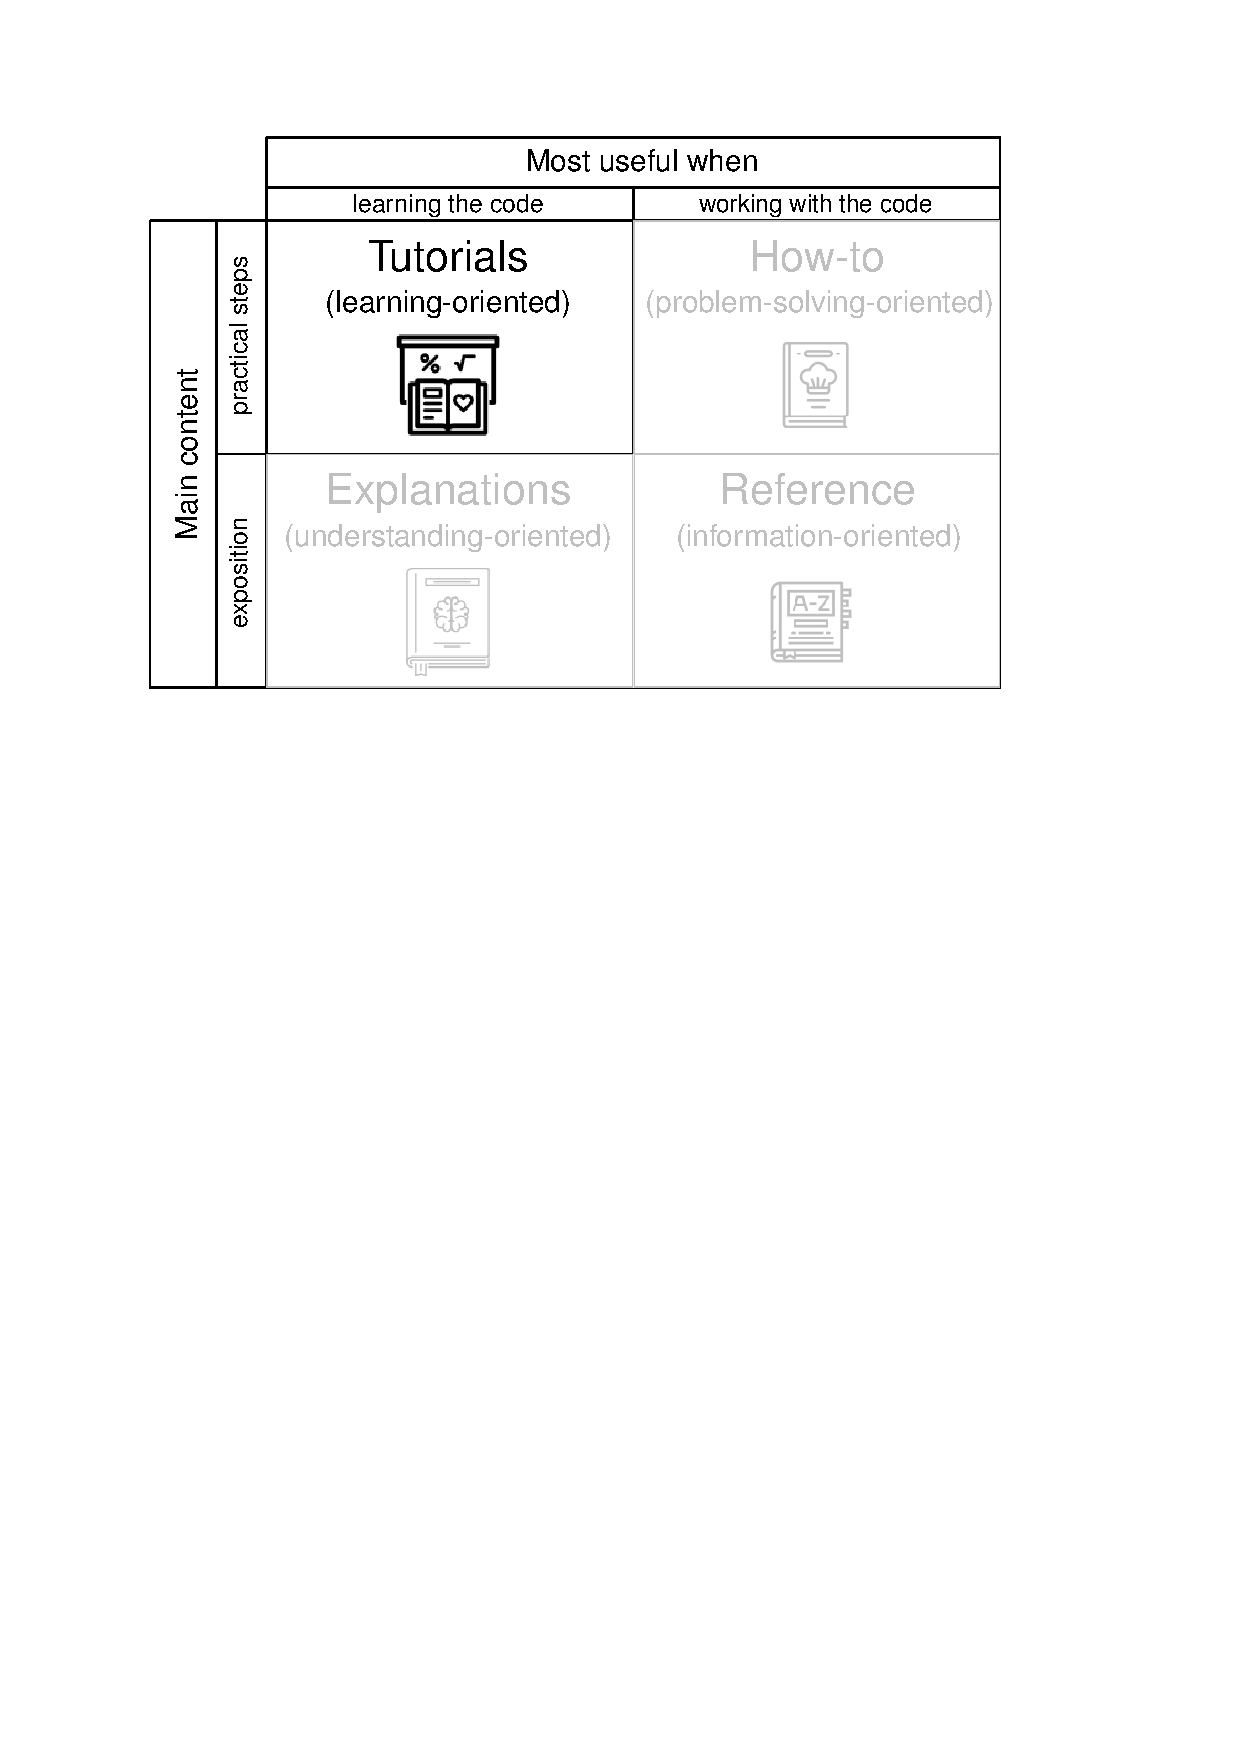
\includegraphics[width=0.9\textwidth]{./figures/documentation-system-tutorials}
    \end{center}
    \begin{exampleblock}{}
        \centering
        Good example: TensorFlow tutorials
        (\url{www.tensorflow.org/tutorials})
    \end{exampleblock}
\end{column}

\end{columns}

\end{frame}

%==============================================================================
\begin{frame}{How-to guides: problem-solving-oriented docs}
\footnotesize

\begin{columns}[onlytextwidth]

\begin{column}{0.4\textwidth}

\begin{itemize}
    \item Think of how-to guides as \emph{recipes} (in a cookbook)
    \item They contain step-by-step instructions on solving a clearly defined problem
    \item They are context-free; readers know what they want to do,
          they just don't know how to do it
    \item Easier to write; pick a common task in \texttt{minterpy}
          and write down the instructions
\end{itemize}

The \texttt{minterpy} docs distinguishes how-to guides
for users and contributors (Contributors Guides).

\end{column}

\begin{column}{0.6\textwidth}
    \begin{center}
    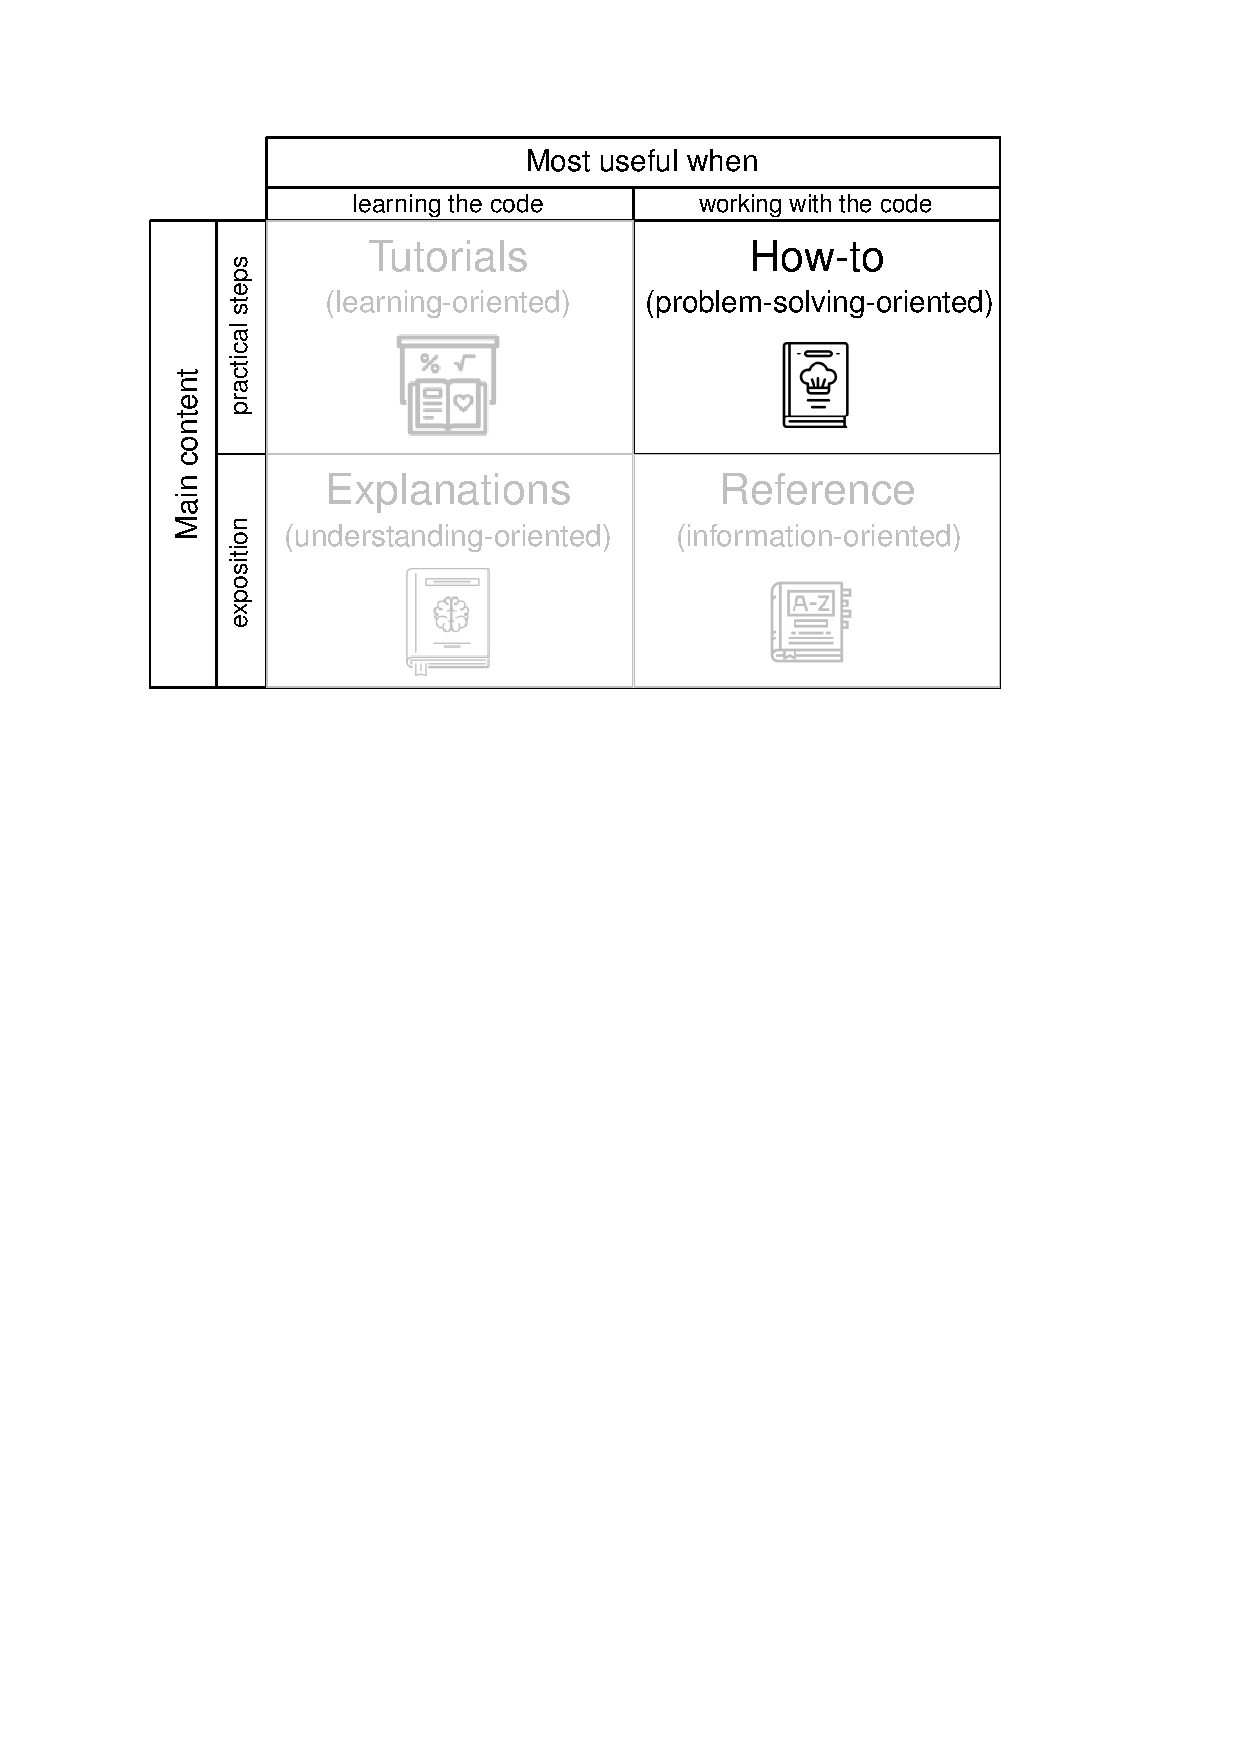
\includegraphics[width=0.7\textwidth]{./figures/documentation-system-how-to}
    \end{center}
    \begin{exampleblock}{}
        \centering
        Good example: The matplotlib Examples
        (\url{matplotlib.org/stable/plot_types/index.html})
    \end{exampleblock}
\end{column}

\end{columns}

\end{frame}

%==============================================================================
\begin{frame}{Explanations/Fundamentals: understanding-oriented docs}
\footnotesize

\begin{columns}[onlytextwidth]

\begin{column}{0.5\textwidth}

\begin{itemize}
    \item Think of explanations as \emph{theoretical expositions} (in a textbook)
    \item They provide context, theoretical foundations,
          and the bridges between different layer of abstractions of \texttt{minterpy}.
    \item They promote users to be better users,
          and contributors to better contributors
    \item Tricky to write: topics are open-ended,
          think well about their depth and curation
\end{itemize}

\end{column}

\begin{column}{0.5\textwidth}
    \begin{center}
    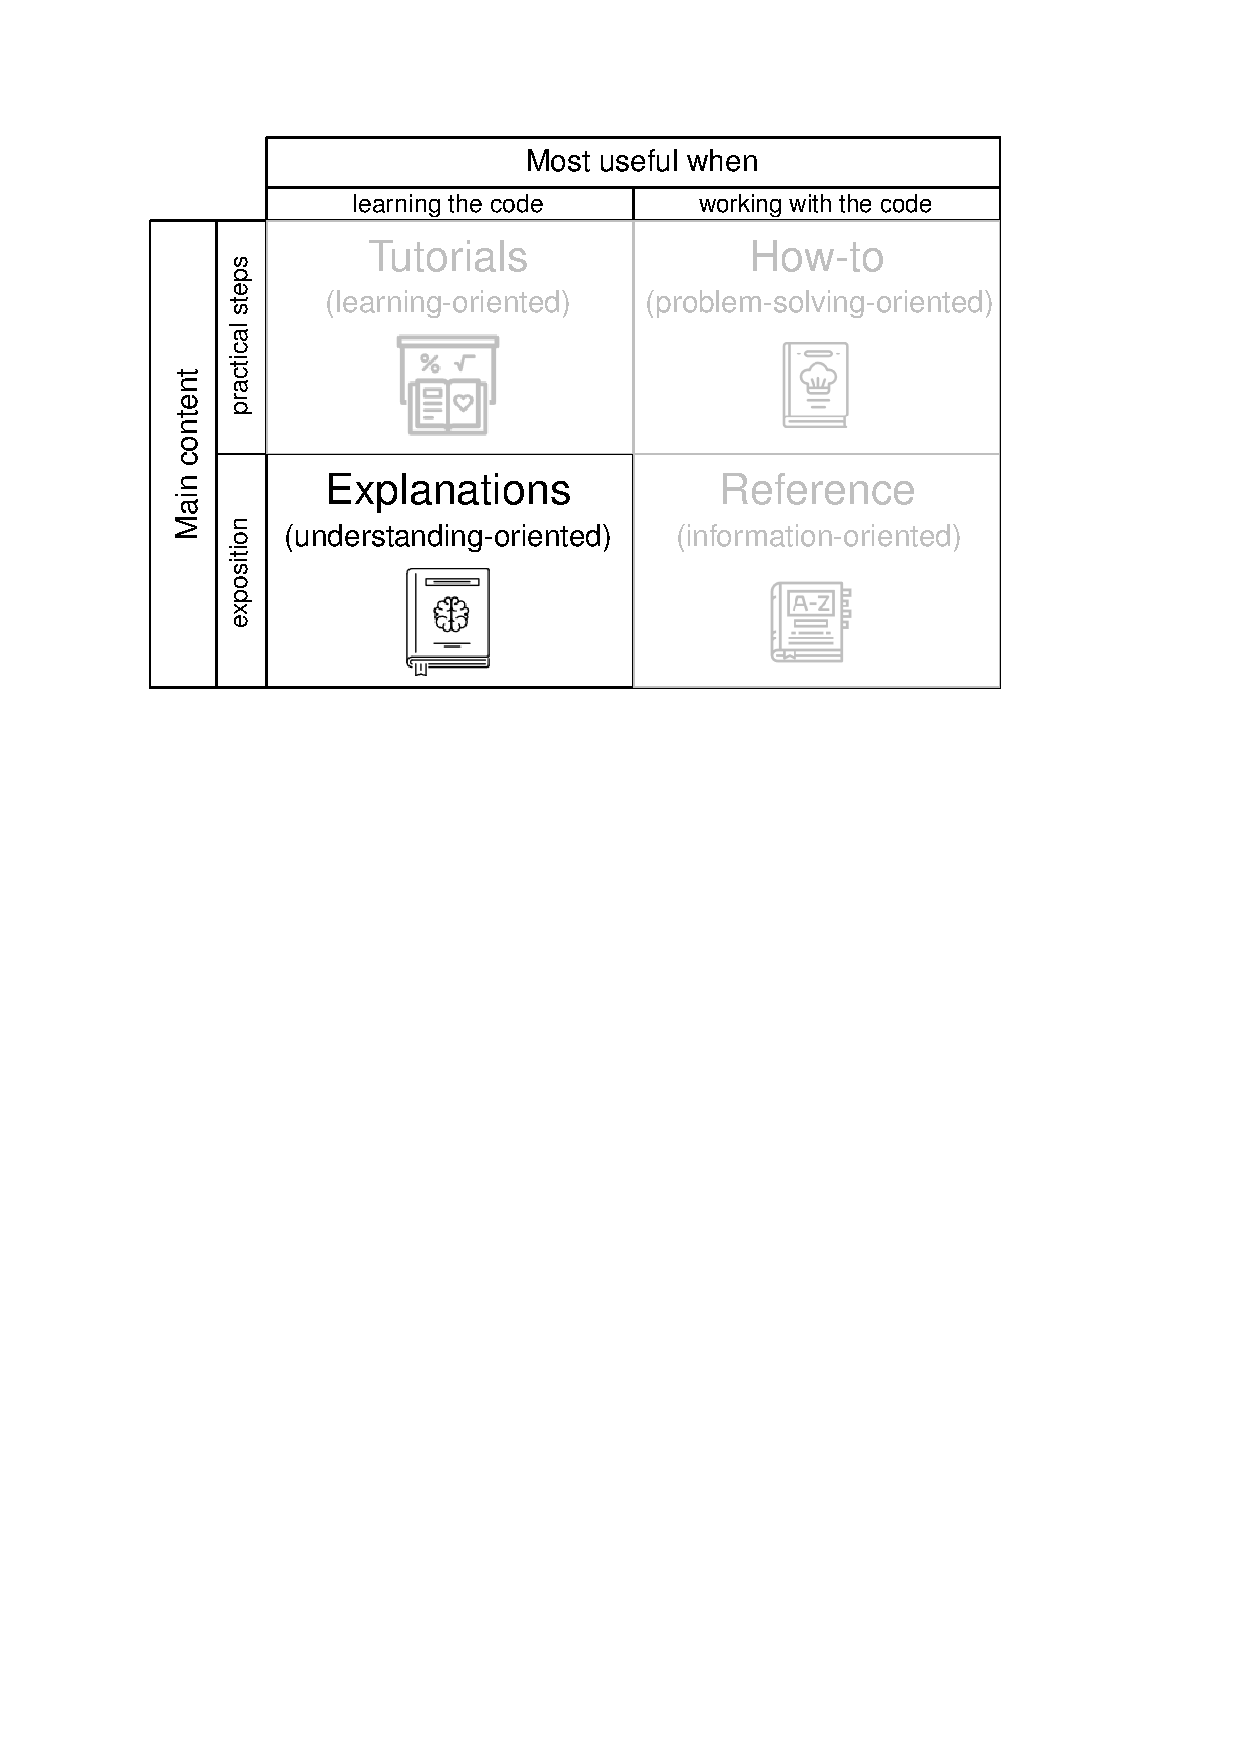
\includegraphics[width=0.9\textwidth]{./figures/documentation-system-explanations}
    \end{center}
\end{column}

\end{columns}

\end{frame}

%==============================================================================
\begin{frame}{API Reference}
\footnotesize

\begin{columns}[onlytextwidth]

\begin{column}{0.5\textwidth}

\begin{itemize}
    \item Think of API reference as \emph{dictionary}
    \item They describe all the exposed components of \texttt{minterpy}
    \item They are important for advanced users and contributors
    \item Easier to write: well-defined and consistent structure,
          (almost) one-to-one corespondence with the codebase
\end{itemize}

\end{column}

\begin{column}{0.5\textwidth}
    \begin{center}
    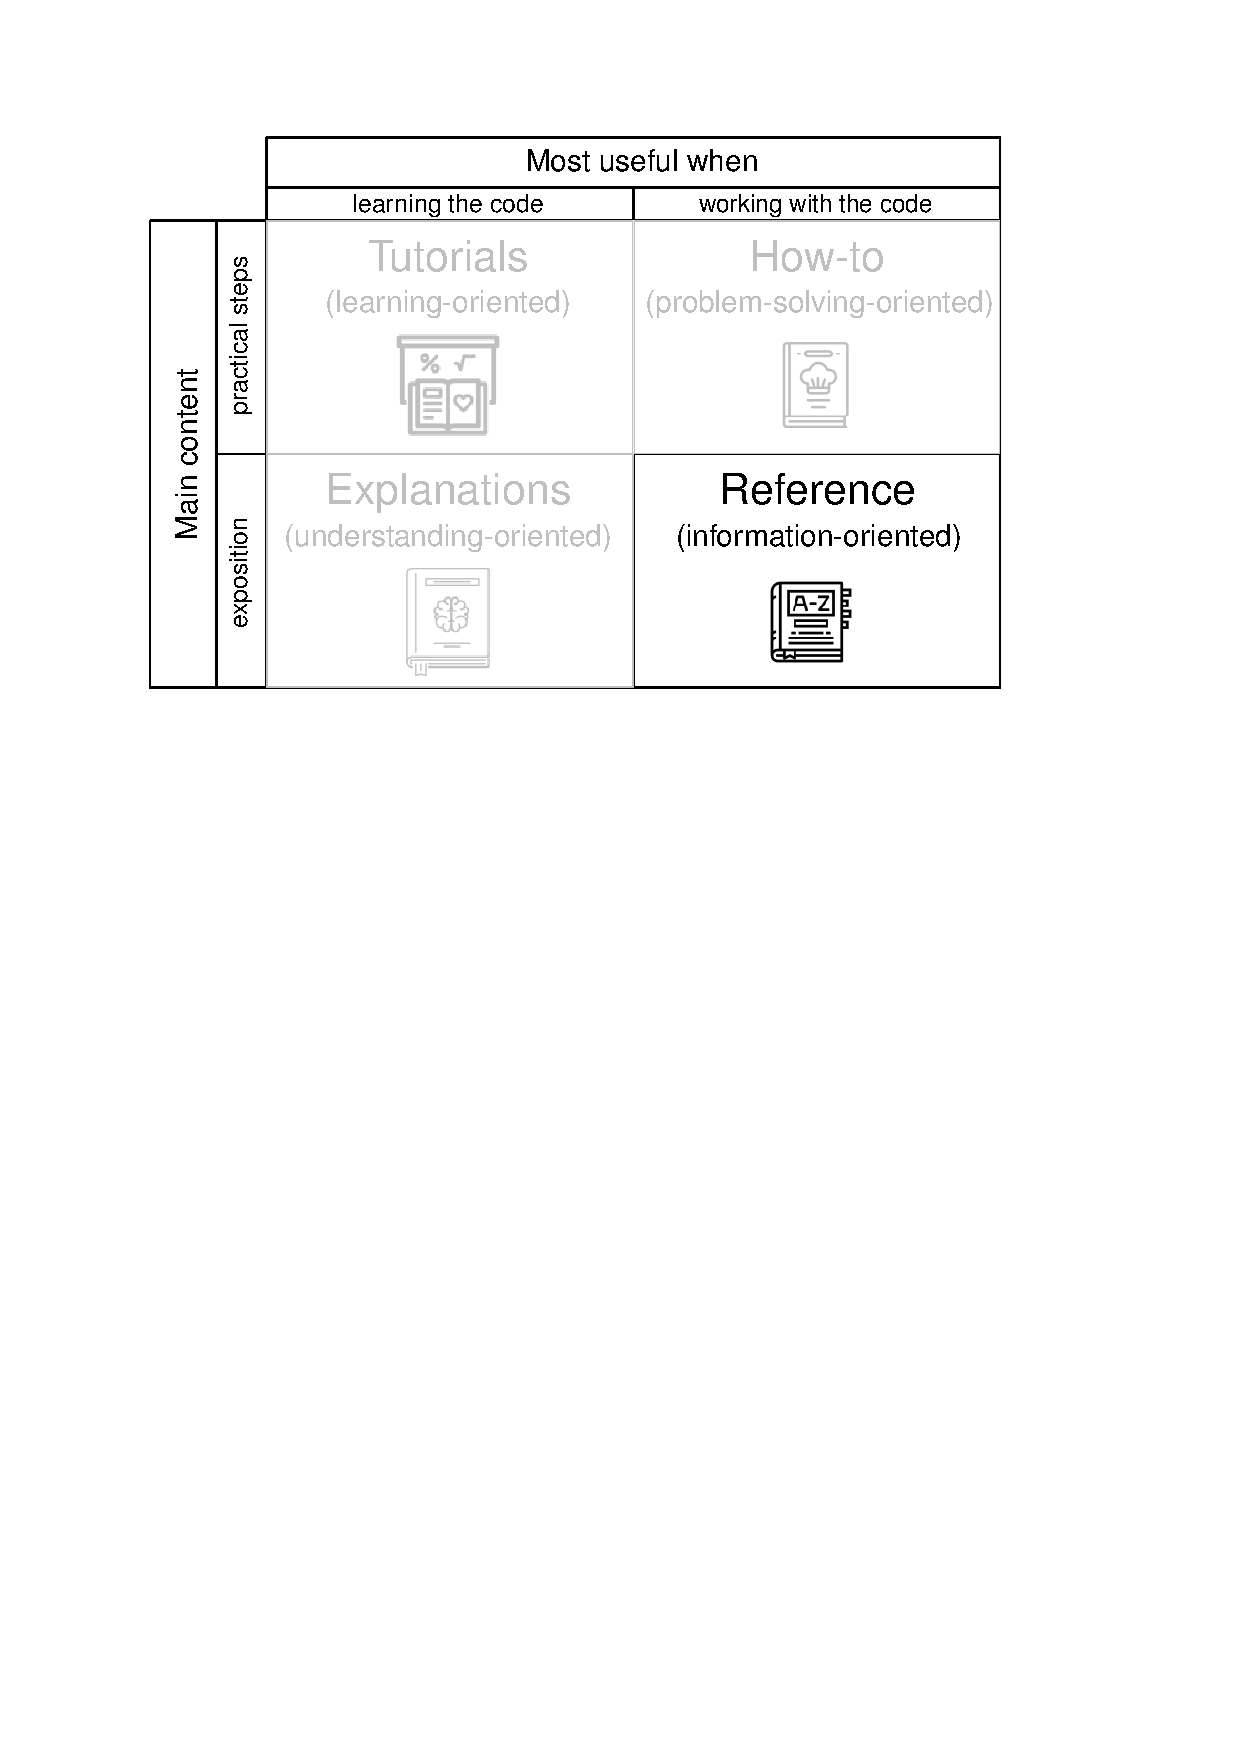
\includegraphics[width=0.9\textwidth]{./figures/documentation-system-reference}
    \end{center}
    \begin{exampleblock}{}
        \centering
        Good example: Most well-known Python packages (NumPy, SciPy, etc.) have a good API reference
    \end{exampleblock}
\end{column}

\end{columns}

\end{frame}


%==============================================================================
\section{Framework and tools}

%==============================================================================
\begin{frame}{Outline}
\tableofcontents[currentsection]
\end{frame}

%==============================================================================
\begin{frame}{Framework: docs-like-code}
\footnotesize

\begin{columns}[onlytextwidth]

\begin{column}{0.5\textwidth}

We write the \texttt{minterpy} docs following the \emph{docs-like-code} framework,
it means that we:

\begin{itemize}
    \item write the docs source files in plain text using a markup language
    \item store the docs source files in a version control system (the same repo as the codebase)
    \item set the workflow for docs contribution is similar to the dev. contribution:
          issues tracker, merge request, and merge review
    \item build the docs artifacts automatically and publish them online
\end{itemize}

\end{column}

\begin{column}{0.5\textwidth}
    \begin{center}
    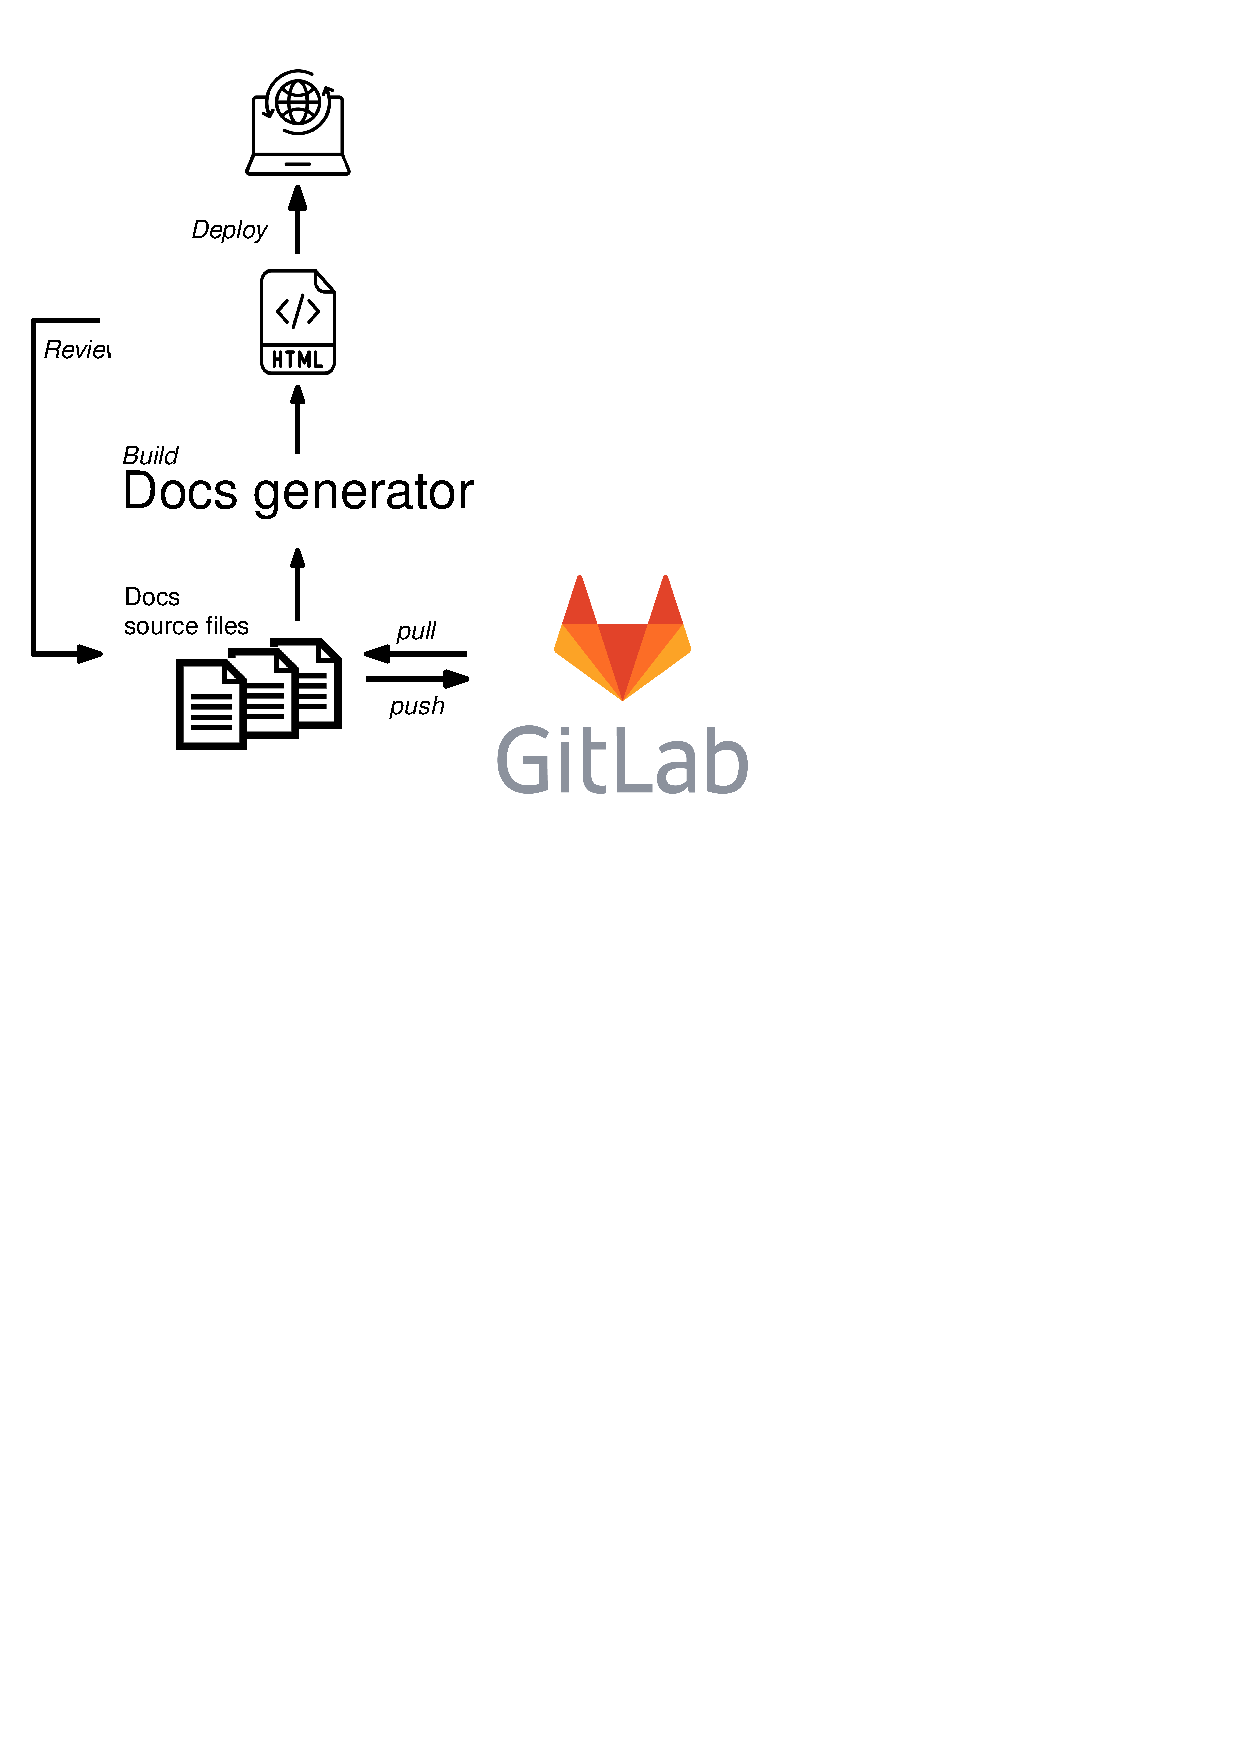
\includegraphics[width=0.9\textwidth]{./figures/documentation-docs-like-code}
    \end{center}
\end{column}

\end{columns}

\end{frame}

%==============================================================================
\begin{frame}{Tooling for the Docs}
\footnotesize

\begin{columns}[onlytextwidth]

\begin{column}{0.5\textwidth}

In practice, we use the Sphinx documentation generator to build the docs.

There are three document types to maintain:

\begin{itemize}
    \item reStructuredText (reST) files (\texttt{.rst}), for most of the docs
    \item Jupyter notebooks (\texttt{.ipynb}),
          for docs with many code examples (tutorials, how-to)
    \item Python docstrings (\texttt{.py}), for the API reference; written in reST syntax
\end{itemize}

We are most probably going to use Read The Docs to serve the docs online (TBD).

\end{column}

\begin{column}{0.5\textwidth}
    \begin{center}
    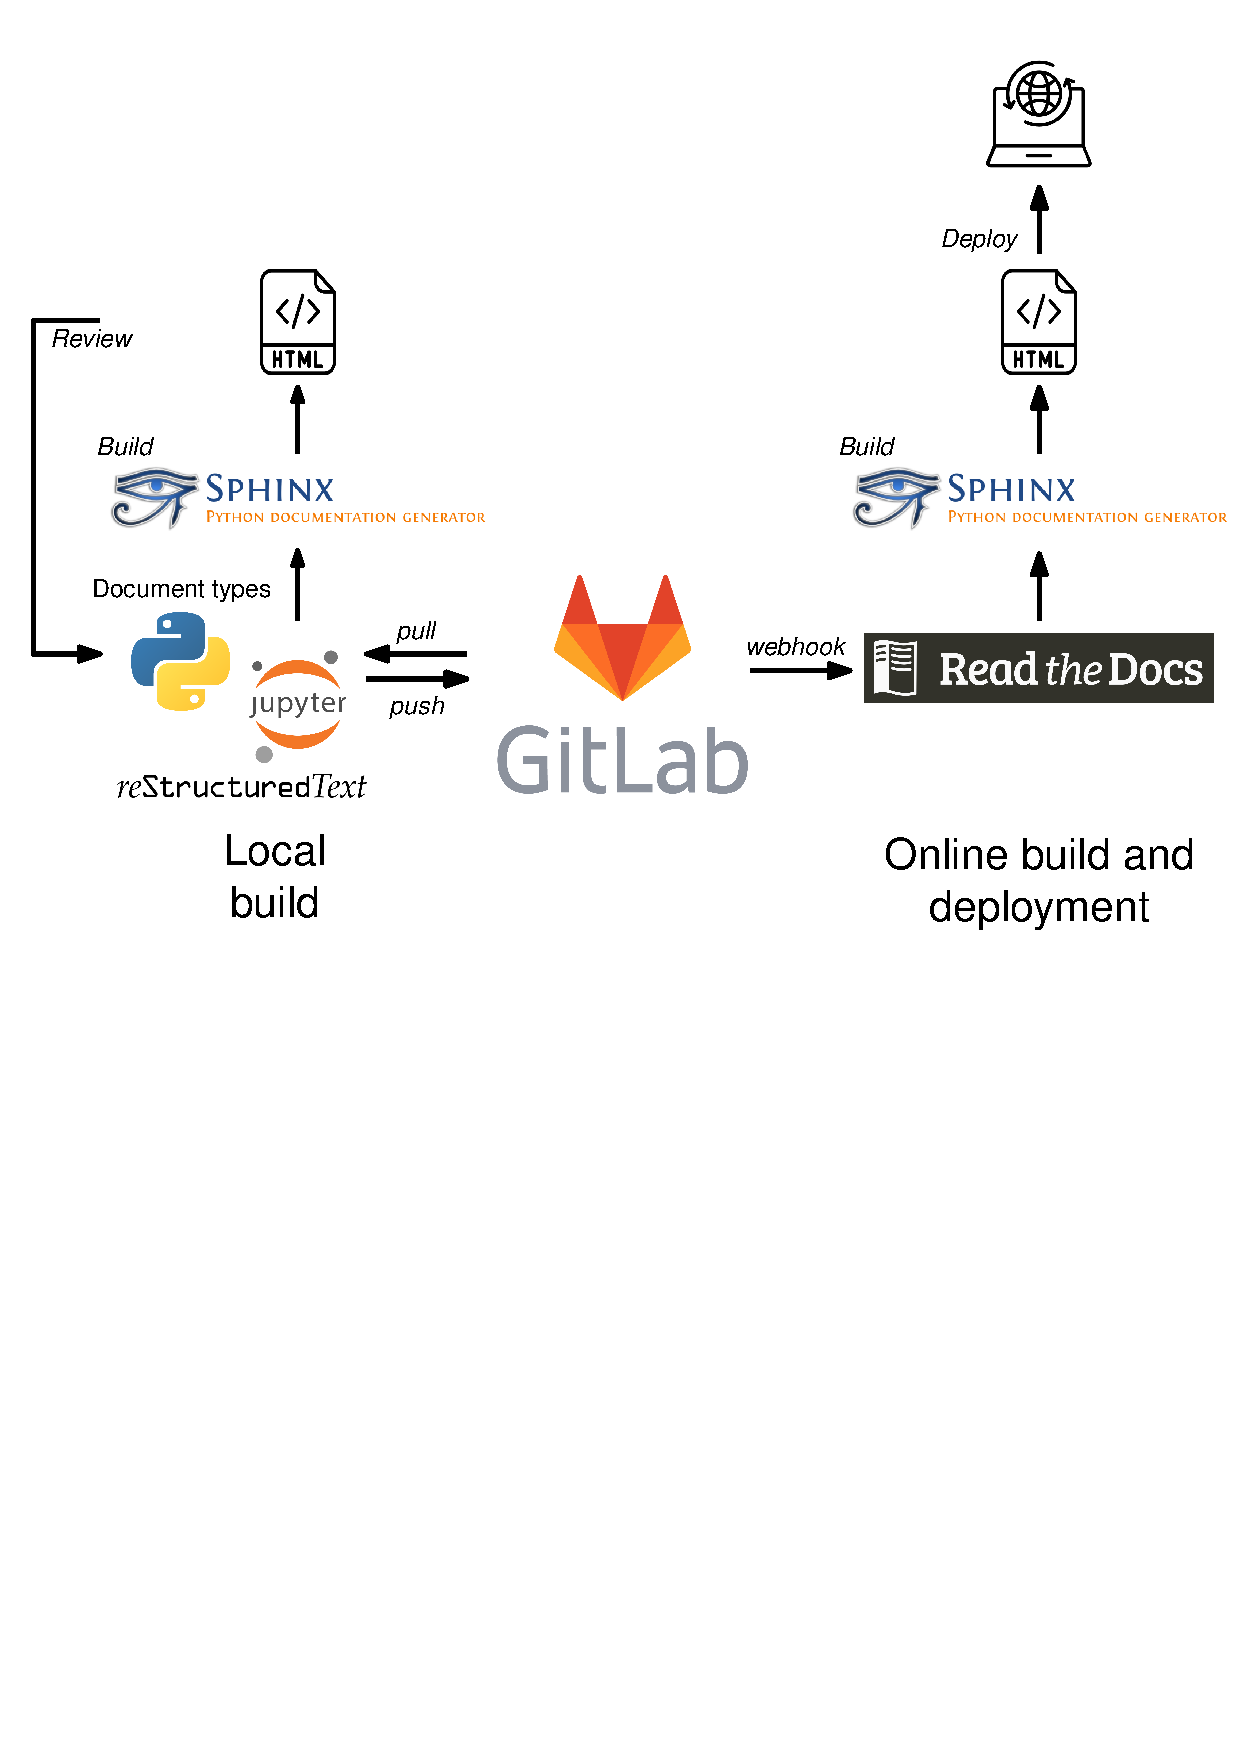
\includegraphics[width=0.9\textwidth]{./figures/documentation-tooling}
    \end{center}
\end{column}

\end{columns}

\end{frame}

%==============================================================================
\section{What you can do to help}

%==============================================================================
\begin{frame}{Outline}
\tableofcontents[currentsection]
\end{frame}
    
%==============================================================================
\begin{frame}{What you can do to help}
\footnotesize

\begin{block}{If you're a \texttt{minterpy} user}
\begin{itemize}
    \item Fix typos and grammatical mistakes (general improvement)
    \item Fix technical errors and inaccuracies
    \item Add new tutorials and how-to guides that you think important but still missing
\end{itemize}

\vspace{0.25em}

Open a new issue, let someone else do it or do it yourself and then do a merge request.
\end{block}

\begin{block}{If you're developing a feature for \texttt{minterpy}}

You're responsible for the docs of your feature;
you should include the docs of each category in your eventual merge request.

\vspace{0.5em}

The docs will also be reviewed.
\end{block}

\end{frame}

%==============================================================================
\begin{frame}{Summary}
\footnotesize

\begin{block}{There are four categories of docs}
\begin{itemize}
    \item Tutorials (Getting Started Guides)
    \item How-to Guides (Users and Contributors)
    \item Fundamentals
    \item API Reference
\end{itemize}
\end{block}

\begin{block}{Docs are maintain like the codebase}
Contribution workflow similar to the workflow for the dev. Three types of document are maintained:
\begin{itemize}
    \item reStructuredText (most of the docs)
    \item Jupyter notebooks (tutorials and how-to)
    \item Python docstrings (API reference)
\end{itemize}
\end{block}

\begin{exampleblock}{}
    \centering
    \textbf{Thank you very much for your attention!}
\end{exampleblock}

\end{frame}


\end{document}

%% 
%% Copyright (C) 2019 by Tobias Schlemmer <Tobias.Schlemmer@web.de>
%% 
%% This work may be distributed and/or modified under the
%% conditions of the LaTeX Project Public License (LPPL), either
%% version 1.3c of this license or (at your option) any later
%% version.  The latest version of this license is in the file:
%% 
%% http://www.latex-project.org/lppl.txt
%% 
%% This work is "maintained" (as per LPPL maintenance status) by
%% Tobias Schlemmer.
%% 
%% This work consists of the file CASUS.dtx and a Makefile.
%% Running "make" generates the derived files
%% 
%% • README,
%% • beamerthemeCASUS.pdf,
%% • beamerthemeCASUS.sty,
%% • beamercolorthemeCASUS.sty,
%% • beamerfontthemeCASUS.sty,
%% • beamerinnerthemeCASUS.sty,
%% • beamerouterthemeCASUS.sty,
%% • CASUSbase.sty,
%% • CASUScolors.sty and
%% • minimalexample.tex
%% • demo169.tex
%% 
%% Running "make inst" installs the files in the user's TeX tree.
%% Running "make install" installs the files in the local TeX tree.
%% 
%% The distribution contains graphics files that are subject to their own
%% license.
%% 
%%
%% End of file `minimalexample'.
